\documentclass[twoside,numberorder]{zjuthesis}
%==============================================================
%==============================================================

%自己需要增加什么 package 或修改什么设置的话,都放在这里吧。
\usepackage{url}
\usepackage{subfigure}

%一些全局工具的定义
\DeclareMathOperator*{\argmin}{arg\,min}
\DeclareMathOperator*{\argmax}{arg\,max}

%==============================================================
%==============================================================
\begin{document}
%==============================================================
%==============================================================
%这部分是论文封面、题名页需要的信息,请根据《研究生学位论文编写规则》自行修改

  %论文题目:{中文}{英文}
  \zjutitle{基于时空正则化的机器学习算法研究}%
           {Learning with Spatial-Temporal Regularization}
  %作者:{中文姓名}{英文}{学号}
  \zjuauthor{张驰原}{Chiyuan Zhang}{3053027068}
  %指导教师:{导师中文名}{导师英文名}
  \zjumentor{何晓飞}{Xiaofei He}
  %个人信息:{年级}{专业名称}
  \zjuinfo{2005 级}{计算机科学与技术}
  %学院信息:{学院中文}{学院英文}{subject}
  \zjucollege{计算机学院}{College of Computer Science}{Machine Learning}
  %日期:{Submitted Date}
  \zjudate{June 1, 2009}

%==============================================================
% 这部分除了“取舍”外,不需要自己修改,必要信息都已在上面设置。

  %封面
  %%============================================================
%% 中文封面

\thispagestyle{empty}

\vspace{5mm}

\begin{center}
   
\includegraphics[width=108mm]{images/zjdx}
\end{center}

\centerline{\songti\erhao\textbf{本科生毕业论文(设计)}}

\vspace{4mm}

\begin{center}
  
\includegraphics[width=35mm]{images/standxb}
\end{center}

\vspace{25mm}

\begin{tabbing}
\hspace{16mm}\songti\sanhao\bfseries 题目: \= \hspace{0mm} \= \parbox[t]{98mm}{%
  \begin{picture}(0,0)(0,0)
  \setlength{\unitlength}{1cm}
    \put(0,-0.2){\line(1,0){9.8}}
  \end{picture}%
\linespread{1.1}\bfseries\Large\zjutitlec} \\[3mm]
\end{tabbing}

\vspace{4mm}

\begin{tabbing}
    \hspace{30mm} \songti\sihao 姓 \hspace{-2.7mm} \= \songti\sihao 名与学号: \= \underline{\makebox[6cm]{\sihao\zjuauthornamec\hspace{3mm}\zjuauthorid}} \\[2mm]
              \> \songti\sihao 指导教师: \> \underline{\makebox[6cm]{\sihao\zjumentorc}} \\[2mm]
              \hspace{30mm} \songti\sihao 年 \hspace{-2.7mm} \= \songti\sihao 级与专业: \= \underline{\makebox[6cm]{\sihao\zjugrade\hspace{3mm}\zjumajor}} \\[2mm]
              \> \songti\sihao 所在学院: \> \underline{\makebox[6cm]{\sihao\zjucollegec}}
\end{tabbing}


%%============================================================
% empty page for two-page print
\ifthenelse{\equal{\zjuside}{T}}{%
  \newpage\mbox{}%
  \thispagestyle{empty}}{}

%%============================================================
%% English Cover
\newpage
\thispagestyle{empty}

\vspace{5mm}

\begin{center}
    \songti\xiaoyi A Dissertation Submitted to Zhejiang University for the Degree of Bachelor of Engineering
\end{center}

\vspace{4mm}

\begin{center}
  
\includegraphics[width=35mm]{images/standxb}
\end{center}

\vspace{25mm}

\begin{tabbing}
\hspace{8mm}\songti\sanhao\bfseries TITLE: \= \hspace{0mm} \= \parbox[t]{124mm}{%
  \begin{picture}(0,0)(0,0)
  \setlength{\unitlength}{1cm}
    \put(0,-0.2){\line(1,0){12.4}}
  \end{picture}%
\linespread{1.1}\bfseries\Large\zjutitlee} \\[3mm]
\end{tabbing}

\vspace{4mm}

\begin{tabbing}
    \hspace{18mm} \= \sanhao Author:\hspace{19mm} \= \underline{\makebox[8cm]{\sanhao\zjuauthornamee\hspace{3mm}\zjuauthorid}} \\[2mm]
                  \> \sanhao Supervisor: \> \underline{\makebox[8cm]{\sanhao\zjumentore}} \\[2mm]
                  \> \sanhao Subject: \> \underline{\makebox[8cm]{\sanhao\zjusubject}} \\[2mm]
                  \> \sanhao College: \> \underline{\makebox[8cm]{\sanhao\zjucollegee}} \\[2mm]
                  \> \sanhao Submitted Date: \> \underline{\makebox[8cm]{\sanhao\zjusubmitteddatee}}
\end{tabbing}

%%============================================================
% empty page for two-page print
\ifthenelse{\equal{\zjuside}{T}}{%
  \newpage\mbox{}%
  \thispagestyle{empty}}{}

  %诚信承诺书
  %% 独创性声明

\newpage
\thispagestyle{empty}

{\songti
\begin{center}
\xiaoer 浙江大学研究生学位论文独创性声明
\end{center}

\vspace{5mm}

本人声明所呈交的学位论文是本人在导师指导下进行的研究工作及取得的研究成果。除了文中特别加以标注和致谢的地方外,论文中不包含其他人已经发表或撰写过的研究成果,也不包含为获得\underline{\kaiti\bfseries\sihao~浙江大学~}或其他教育机构的学位或证书而使用过的材料。与我一同工作的同志对本研究所做的任何贡献均已在论文中作了明确的说明并表示谢意。

\begin{tabbing}
\hspace{0.5\linewidth} \= \hspace{0.5\linewidth} \kill \\
学位论文作者签名: \> 签字日期: \quad\quad\quad 年\quad\quad 月\quad\quad 日
\end{tabbing}

\vspace{20mm}

\begin{center}
\xiaoer 学位论文版权使用授权书
\end{center}

\vspace{5mm}

本学位论文作者完全了解\underline{\kaiti\bfseries\sihao~浙江大学~}有权保留并向国家有关部门或机构送交本论文的复印件和磁盘,允许论文被查阅和借阅。本人授权\underline{\kaiti\bfseries\sihao~浙江大学~}可以将学位论文的全部或部分内容编入有关数据库进行检索和传播,可以采用影印、缩印或扫描等复制手段保存、汇编学位论文。

(保密的学位论文在解密后适用本授权书)

\begin{tabbing}
\hspace{0.5\linewidth} \= \hspace{0.5\linewidth} \kill \\
学位论文作者签名: \> 导师签名: \\[5mm]
签字日期: \quad\quad\quad 年\quad\quad 月\quad\quad 日 \> 签字日期: \quad\quad\quad 年\quad\quad 月\quad\quad 日
\end{tabbing}
}

\ifthenelse{\equal{\zjuside}{T}}{%
  \newpage\mbox{}%
  \thispagestyle{empty}}{}


  \frontmatter   
  \pagenumbering{Roman}

  %中文摘要
  %% 中文摘要
\chapter*{\centerline{摘\quad 要}}
\chaptermark{摘要}
\addcontentsline{toc}{chapter}{摘要}

\vspace{1em}

这是一篇有关法器钉耙的研究。以往法器研究都是从西方视角出发,没有考虑东方文化背景的影响。本研究结合钉耙在农业中的广泛应用,对钉耙的作用进行开创性研究。

扯几句,再扯几句。

\vspace{1em}

\noindent\textbf{关键词:钉耙\quad 成本\quad 法器}

  %英文摘要
  %% 英文摘要
\chapter*{\centerline{Abstract}}
\chaptermark{Abstract}
\addcontentsline{toc}{chapter}{Abstract}

\vspace{1em}
Most of the machine learning tasks can be regards as finding a
function/model $f$ that minimize the empirical risk. But that will
work well only when you have enough training data. While people
start to pay attention to learning problems with very few training
data, regularization becomes more and more important. With
additional regularizer added to the original objective function, one
can restrict the class of admissible solutions to increase the
\textit{generalization performance}. However, most of the
regularization techniques proposed haven't take special attention to
the temporal property of the problem. Considering the large amount
of data evolving with time (e.g. dynamic web pages, blog contents
and stock prices), we propose a novel regularizer that considers
both spatial and temporal smoothness over the data. We apply our
algorithm in the problem of video compress. The experimental results
demonstrate the effectiveness of the proposed algorithm.

\vspace{1em}

\noindent\textbf{Keywords}:~~Machine Learning,~~Regularization,~~Video Compression


%==============================================================
%这部分不需要自己修改。

  %目次页
  \tableofcontents
  \chaptermark{目录}
  \addcontentsline{toc}{chapter}{目录}

  \mainmatter

%==============================================================

  \chapter{绪论}

\section{机器学习与正则化}

机器学习是人工智能的一个子领域,它着眼于设计和开发能自动从数据中生成出模型的算法。机器学习又
被细分为监督学习、无监督学习以及半监督学习、增强学习等类别,但是它们的思路都是相似的,亦即对
问题进行建模,并寻找一个最适合给定约束条件的函数或模型,通常约束条件直接来自于训练数据。如果
训练数据的数量足够多,我们通常能得到比较好的结果,然而大多数时候训练数据总是不够的,此时我们
通常会遇到有很多(甚至无穷多个)满足约束条件的解的情况,并且大部分这样的解在未知数据上的表现
非常差。换句话说,这样的问题是数值不稳定的,或者说泛化性能很差。

一种解决办法就是正则化(Regularization),亦即对可能解空间进行限制,这种技术最初由
Tikhonov 和 Arsenin \cite{tikhomirov1960dsf} 提出,用于解决矩阵求逆的问题,并且后
来被成功地应用到机器学习中来。许多机器学习的算法(例如支持向量机)都可以看成是某
种形式的正则化。简单来说,正则化可以看作是关于待解决问题的某种先验的知识,例如,在
脊回归(Ridge Reguression)中的正则化可以看作是将参数的先验分布定为高斯分布的结果,
而流形正则化(Manifold Regularization)\cite{On-Manifold-Regularization} 则是编码了
数据点都分布在一个低维流形上这样一个先验假设。

虽然正则化如今已经成为机器学习中广泛使用的一种技术,大多数情况人们都只考虑了问题在空间上的
属性。当我们遇到随时间变化的数据(例如,动态网页、博客内容或者股票价格等)时,一个很自然的
想法就是要保证数据在时间上的平滑性,这样的假设通常能帮助我们得到更健壮的解。

\section{时空正则化与视频压缩}

\begin{figure*}
\center{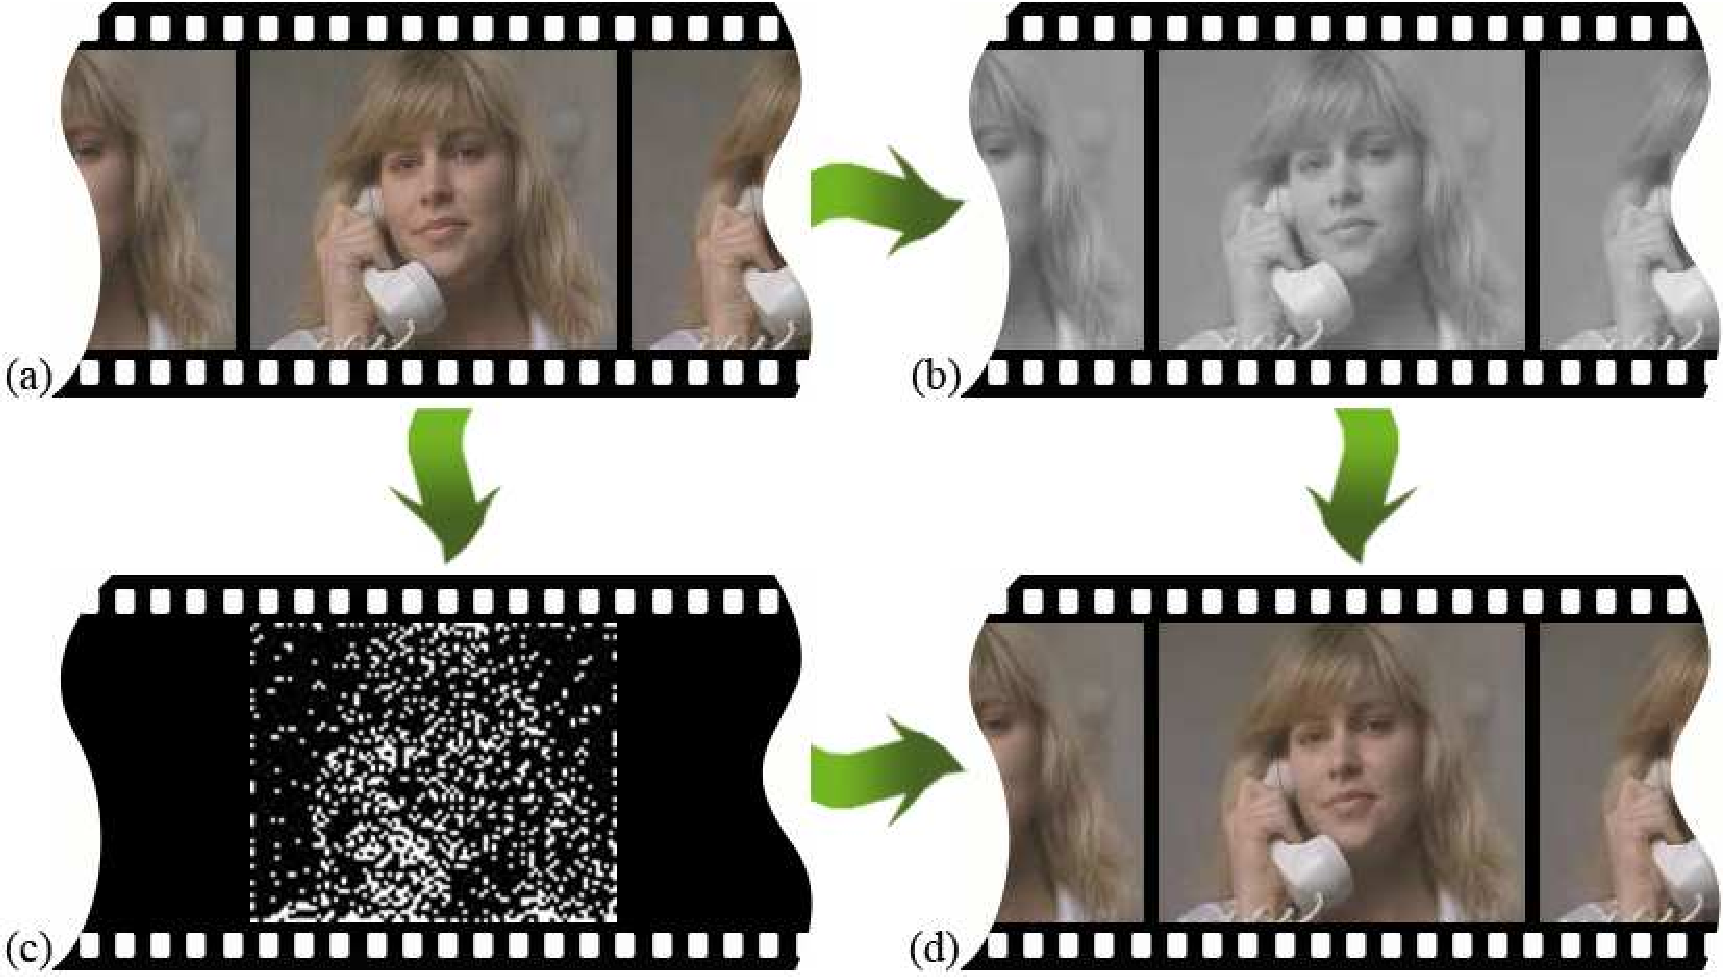
\includegraphics[width=380pt]{images/cycle}}
\caption{\label{fig:cycle}基于学习的视频压缩的例子。 (a) 原始视频帧
(b) 灰度帧 (c) 选取的带有颜色信息的点 (d) 恢复的视频帧}
\end{figure*}

在本文中,我们将从视频压缩这个具体的例子出发,来阐述同时结合时间和空间的正则化
给机器学习问题所带来的性能提升。
视频是一种典型的随着时间轴变化的数据,并且通常在
时间上的变化是比较平滑的,正好是时空正则化的典型应用场景。视频压缩是一项用于缓解
视频存储空间以及传输带宽占用的
关键性技术。视频数据通常包含了许多时间和空间上的冗余信息。相似信息可以通过编码帧内
(空间上的)或帧间(时间上的)差异的方式来进行存储。
典型的压缩方法包括了离散余弦变换、 向量化、分形压缩以及离散小波变换等。

最近 \cite{learning-to-compress-images}
提出了基于机器学习的视频压缩方法。他们提出了和传统的频域转换不同的方式,将原始的带颜色的视频
转化为一个灰度视频,选取一些有代表性的点并存储他们的颜色信息,然后使用灰度视频和带有颜色信息
的点学习出一个统计模型,用于预测其他像素点的颜色值。实验结果表明,在保证图像质量(通过
PSNR
\footnote{http://en.wikipedia.org/wiki/PSNR}进行衡量)的前提下,可以达到不错的压缩效果。

从机器学习的视角来看,这里主要有两个基本的问题。首先是如何选取最有代表性的点,这本质上是一个
主动学习(Active
Learning)的问题。存储灰度视频和选出来的颜色点的信息就是编码的过程。
其次是如何结合选出来的带颜色信息的点和灰度视频来学习一个模型,这在本质上是
一个半监督学习(Semi-supervised
Learning)的问题。用这个模型来恢复原始视频就是解码的过程。在这里有颜色的像素被当作是带标签的
数据,而灰度像素则被当作是无标签的数据。\cite{learning-to-compress-images}
使用了一种非常直接的主动学习的方法:在每一次迭代的时候简单地在预测错误率最高的区域选点。在选
点之后他们使用拉普拉斯正则化的最小二乘法(LapRLS,\cite{Manifold-Regularization-Journal})来
完成半监督学习的问题。他们的方法的最大的不足就是没有任何理论上的依据可以保证使用这种方法选出来
的点可以降低预测的错误率。

在本文中,我们将提出一个针对视频压缩的自主学习和半监督学习的统一框架,并使用时空正则化的方法
对其进行改进以获得性能提升。我们的方法的中心思想是颜色
点的选取和后续的着色过程应该同时进行优化。具体来讲,对于着色的过程,我们假定每个像素的颜色值可以
通过其(时间或空间上的)邻居中灰度值相似的像素的颜色值重新构造出来,并使用正则化的最小二乘法
来学习一个模型;对于选点的过程,我们使用相同的损失函数(loss
function),并使用最小化系数的协方差矩阵的准则来进行选点。然后我们还讨论了如何将自主学习和半监督
学习结合起来应用到视频压缩上面。学习出来的模型不仅用于预测当前的帧,而且还被用于预测后续的相似的
帧,知道 PSNR 分值降低超过了一定的阈值,再重新训练一个模型。图
\ref{fig:cycle} 展示了我们的方法是如何工作的。

论文余下的部分是这样组织的:在第二章中,我们简要地回顾了一下这个领域相关的工作。用于着色的半监督
学习的办法将会在第三章中介绍。第四章介绍如何通过主动学习选取最具代表性的点。然后我们会在第五章中
给出一个用于视频压缩的主动学习和半监督学习的统一框架并运用时空正则化的方法进行改进。实验结果将在
第六章中展示。第七章我们将会进行简要总结并展望后续的工作。


  
\chapter{第二章}

这是第二章,目的是占个位置。你知道《浙大同学爱占坐》这首歌吗?
  \chapter{基于半监督学习的着色}
\label{chap:semi-supervised-learning}

在本章中,我们将介绍一种全新的使用半监督学习进行着色的方法。这个方法的基本假设是:每个像素点的颜色值可以由
在时空上邻近并且灰度值相似的像素点的颜色值重新构造出来。这个算法灵感来源于一些前人的工作
\cite{Manifold-Regularization-Journal,LLE,NPE}.

\section{算法}

我们用位置和灰度值来表示图像中的每一个像素。这样,每个像素可以由一个向量$\textbf{x}
\in
\mathbb{R}^d$来表示。和LapRLS类似,我们在像素点$\textbf{x}_1,
\cdots,
\textbf{x}_m$上构造一个邻接图$G$。为了获取这些点之间的关系,我们对如下的图上的正则化损失函数进行最小化:

\begin{equation}\label{eqn:regularized-regression}
    \mathcal{L}(f)= \sum_{i=1}^k \big( y_i - f(\mathbf{x}_i) \big)^2 + \lambda J(f),
\end{equation}

其中$J(f)$控制了假设空间的学习复杂度,系数$\lambda$控制了实验误差和模型复杂度之间的平衡性。

对于普通的图片,通常一个像素点的位置和灰度值都可以根据其相邻的像素估计出来。因此,我们将每个像素用其邻接
点线性表示出来,并使用这些线性系数来表征数据点之间的关系。重新构造所产生的误差由如下的损失函数来进行度量
\cite{LLE}:

$$
\phi (W) = \sum_{i=1}^{m} \| \mathbf{x}_i - \sum_{j=1}^{m} W_{ij}
\mathbf{x}_j \|^2,
$$

这个损失函数将每个数据点到它重新构造出来的值之间的距离的平方累加起来。需要注意的是,如果$\textbf{x}_i$和
$\textbf{x}_j$之间没有连接起来,$W_{ij}$将会等于零。这个代价函数最初是在\textit{局部线性嵌入}算法中用于
学习数据空间的几何结构的,详见\cite{LLE}。

现在考虑估计每个像素点的标签(即颜色值)的问题,我们希望每个像素点的标签也可以经过系数$W_{ij}$由与其相邻
的像素点的标签组合而来。我们认为如下这样的正则化项是合理的,可以用于选取一个较好的模型:

\begin{equation}\label{eqn:regularizer}
    J(f)=\sum_{i=1}^{m} \Big( f(\mathbf{x}_i) - \sum_{j=1}^{m} W_{ij} f(\mathbf{x}_j) \Big)^2.
\end{equation}

需要注意的是,在(\ref{eqn:regularizer})中,权值$W_{ij}$是固定的。对于线性函数$f(\textbf{x})=\textbf{a}^T
\textbf{x}$,(\ref{eqn:regularizer}将变成

\begin{equation}\label{eqn:linear-regularizer}
    J(\mathbf{a})=\sum_{i=1}^{m} \Big( \mathbf{a}^T \mathbf{x}_i -
    \sum_{j=1}^{m} W_{ij} \mathbf{a}^T \mathbf{x}_j \Big)^2.
\end{equation}

通过一些简单的代数变换,我们可以得到:

\begin{eqnarray*}
J(\mathbf{a})&=&\textbf{a}^T \Big( \sum_{i=1}^m \big( \mathbf{x}_i -
\sum_{j=1}^{m} W_{ij} \mathbf{x}_j\big) \big( \mathbf{x}_i -
\sum_{j=1}^{m} W_{ij} \mathbf{x}_j \big)^T \Big) \textbf{a}\\
&=&\textbf{a}^T \big(X-XW^T \big) \big(X-XW^T \big)^T
\textbf{a}\\
   &=& \mathbf{a}^T X(I-W)^T(I-W)X^T \mathbf{a}\\
   &\doteq& \mathbf{a}^T XMX^T \mathbf{a},
\end{eqnarray*}

其中$M=(I_W)^T(I_W)$。易知$M$是对称且半正定的的。令$y_i=f(\mathbf{x}_i)$,$\mathbf{y}
= (y_1, y_2, \cdots, y_k)^T$,则图像的最小平方误差如下:

\begin{eqnarray*}
% \nonumber to remove numbering (before each equation)
&& \sum_{i=1}^l \Big( y_i - \mathbf{a}^T \mathbf{x}_i \Big)^2\\
&=& \Big( \mathbf{y}-Z^T \mathbf{a}\Big)^T \Big( \mathbf{y}-Z^T \mathbf{a}\Big) \\
&=& \mathbf{y}^T \mathbf{y}-2\mathbf{a}^T Z\mathbf{y}+\mathbf{a}^T
ZZ^T \mathbf{a}.
\end{eqnarray*}

注意到$\mathbf{y}^T
\mathbf{y}$是一个常量,因此损失函数(\ref{eqn:regularized-regression})可以被归约为如下
形式:

\begin{equation}\label{eqn:final-loss-function}
    \mathcal{L}(\mathbf{a})= -2\mathbf{a}^T Z\mathbf{y}+\mathbf{a}^T ZZ^T \mathbf{a}
    + \lambda \mathbf{a}^T XMX^T \mathbf{a}.
\end{equation}

零$\mathcal{L}$的导数等于零,我们有:

\begin{eqnarray}
% \nonumber to remove numbering (before each equation)
&& \frac{\partial \mathcal{L}}{\partial \mathbf{a}} =0 \nonumber \\
 &\Rightarrow& -2Z\mathbf{y}+2ZZ^T \mathbf{a}
    + 2\lambda XMX^T \mathbf{a}=0 \nonumber \\
 &\Rightarrow& \mathbf{a}=\Big( ZZ^T + \lambda XMX^T \Big)^{-1}Z\mathbf{y}
 \label{eqn:sol}
\end{eqnarray}

有时候矩阵$ZZ^T+\lambda
XMX^T$可能是奇异的,我们可以添加一个脊正则化项\cite{statistical-leraning}从而得到如下形式:
\begin{equation}
\label{eqn:regularized-regression-linear}
    \mathcal{L}(\textbf{a})= \sum_{i=1}^k \big( y_i - \textbf{a}^T \textbf{x}_i \big)^2 +
    \lambda_1 J(f) + \lambda_2 \|\textbf{a}\|^2,
\end{equation}
新的损失函数的解如下所示:
\begin{equation}
\label{eqn:linear-sol} \mathbf{a}=\Big( ZZ^T + \lambda_1 XMX^T +
\lambda_2 I \Big)^{-1}Z\mathbf{y}
\end{equation}
易知矩阵$ZZ^T + \lambda XMX^T$是半正定的。因此,矩阵$ZZ^T +
\lambda_1 XMX^T + \lambda_2 I$是可逆的。一旦得到了回归函数$f$,任意
像素点$\mathbf{x}$的标签就可以通过$f(\mathbf{x}) = \mathbf{a}^T
\mathbf{x}$估计出来。

\section{非线性推广}
\label{sec:nonlinear-generalization}
在本小节中,我们会讨论使用核方法\cite{Learning-with-Kernels}
来将正则化的回归算法推广到非线性的情况。

我们在关联到一个核函数$\mathcal{K}: \mathbb{R}^d\times \mathbb{R}^d
\rightarrow \mathbb{R}$再生核希尔伯特空间$\mathcal{H}$里来考虑这个
问题。在$\mathcal{H}$里的损失函数可以写成如下形式:
\begin{equation}
\label{eqn:rkhs-obj}
 \mathcal{L}(f)= \sum_{i=1}^k \big( y_i - f(\mathbf{x}_i) \big)^2 +
 \lambda_1 J(f) + \lambda_2 \|f\|_{\mathcal{H}}, f \in \mathcal{H}.
\end{equation}
由representer theorem
\cite{Learning-with-Kernels,Manifold-Regularization-Journal}可知,最
优的$f$具有如下形式:
\begin{equation}
\label{eqn:representer-theorem} f(\textbf{x})=\sum_{i=1}^m \alpha_i
\mathcal{K}(\textbf{x}, \textbf{x}_i)
\end{equation}
令$K_{XX}$为一个$m\times m$的核矩阵,其中$K_{XX,ij}=\mathcal{K}
(\textbf{x}_i, \textbf{x}_j)$,并令$K_{ZX}$为一个$k \times m$的核
矩阵,其中$K_{ZX,ij}=\mathcal{K}(\mathbf{z}_i\mathbf{x}_j)$。我们定义
$$
\textbf{f}_Z=\big( f(\textbf{z}_1), \cdots, f(\textbf{z}_k) \big)^T.
$$
显然$\textbf{f}_Z = K_{ZX} \pmb{\alpha}$,因此
\begin{eqnarray*}
&&\sum_{i=1}^k \big( y_i - f(\textbf{z}_i) \big)^2 = \big(
\textbf{y}
- \textbf{f}_Z \big)^T \big( \textbf{y} - \textbf{f}_Z \big)\\
&=&\big( \textbf{y} - K_{ZX} \pmb{\alpha} \big)^T \big( \textbf{y} -
K_{ZX} \pmb{\alpha} \big)\\
&=&\textbf{y}^T \textbf{y} - 2 \textbf{y}^T K_{ZX} \pmb{\alpha} +
\pmb{\alpha}^T K_{ZX}^T K_{ZX} \pmb{\alpha}
\end{eqnarray*}
类似地,我们定义
$$
\textbf{f}_X=\big( f(\textbf{x}_1), \cdots, f(\textbf{x}_m) \big)^T
= K_{XX} \pmb{\alpha}.
$$
则
\begin{eqnarray*}
J(f)&=&\sum_{i=1}^{m} \Big( f(\mathbf{x}_i) - \sum_{j=1}^{m} W_{ij}
f(\mathbf{x}_j) \Big)^2 \\
&=& \big( K_{XX} \pmb{\alpha} - W K_{XX} \pmb{\alpha} \big)^T \big(
K_{XX} \pmb{\alpha} - W K_{XX} \pmb{\alpha} \big) \\
&=& \pmb{\alpha}^T K_{XX} \big(I-W)^T(I-W) K_{XX} \pmb{\alpha}\\
&=& \pmb{\alpha}^T K_{XX} M K_{XX} \pmb{\alpha}
\end{eqnarray*}
并且
\begin{eqnarray*}
\|f\|^2_{\mathcal{H}}&=&\langle f, f \rangle \\
&=& \langle \sum_{i=1}^m \alpha_i \mathcal{K}(\cdot, \textbf{x}_i),
\sum_{j=1}^m \alpha_j \mathcal{K}(\cdot,
\textbf{x}_j) \rangle \\
&=& \sum_{i,j} \alpha_i \alpha_j \langle \mathcal{K}(\cdot,
\textbf{x}_i), \mathcal{K}(\cdot, \textbf{x}_j) \rangle \\
&=& \sum_{i,j} \alpha_i \alpha_j \mathcal{K} (\textbf{x}_i,
\textbf{x}_j)\\
&=& \pmb{\alpha}^T K_{XX} \pmb{\alpha}
\end{eqnarray*}
这样,损失函数可以被化简为
\begin{eqnarray*}
\mathcal{L}(f)&=&\textbf{y}^T \textbf{y} - 2 \textbf{y}^T K_{ZX}
\pmb{\alpha} + \pmb{\alpha}^T K_{ZX}^T K_{ZX} \pmb{\alpha}\\
&& + \lambda_1 \pmb{\alpha}^T K_{XX} M K_{XX} \pmb{\alpha} +
\lambda_2 \pmb{\alpha}^T K_{XX} \pmb{\alpha}
\end{eqnarray*}
令$\mathcal{L}$的导数等于零,则得到如下形式的解:
\begin{equation}
\label{eqn:kernel-regression-sol} \pmb{\alpha}=\big( K_{ZX}^T K_{ZX}
+ \lambda_1 K_{XX}M K_{XX} + \lambda_2 K_{XX} \big)^{-1} K_{ZX}^T
\textbf{y}
\end{equation}


  \chapter{基于主动学习的选点}

基于机器学习的视频压缩中关键性的一个步骤就是选取最具有代表性的点。在本
节中我们将会介绍一种基于主动学习的选点方法。这种主动学习的方法使用的损
失函数和上一小节中介绍的半监督学习算法的损失函数完全相同。具体地说,我
们希望使用这种方法选出来的点用于训练可以最小化预测误差。

\section{Bias和Variance的分析}

因为$y_i=\textbf{a}^T \mathbf{z}_i+\epsilon$,我们有$\mathbf{y}=Z^T
\mathbf{a}+\pmb{\epsilon}$,其中$\pmb{\epsilon}=(\epsilon, \cdots,
\epsilon)^T$。显然$E(\pmb{\epsilon}) = \mathbf{0}$,其
中$\mathbf{0}=(0,\cdots,0)$。我们定义
\begin{equation}\label{eqn:hessian-LapRLS}
H=ZZ^T + \lambda_1 XMX^T + \lambda_2 I
\end{equation}
\begin{equation}\label{eqn:lambda-LapRLS}
\Lambda=\lambda_1 XMX^T + \lambda_2 I.
\end{equation}
其中$H$是损失函数的黑塞矩阵。系数向量$\mathbf{a}$的估计值的bias可
以由以下的式子计算出来:
\begin{eqnarray}
% \nonumber to remove numbering (before each equation)
&& E(\widehat{\textbf{a}}-\textbf{a})=E(H^{-1}Z\textbf{y})-\textbf{a} =H^{-1}Z E(\textbf{y})-\textbf{a}\nonumber \\
&=& H^{-1}ZZ^T\textbf{a}-\textbf{a} = H^{-1}(ZZ^T + \Lambda - \Lambda)\textbf{a}-\textbf{a} \nonumber \\
&=& (I-H^{-1} \Lambda)\textbf{a}-\textbf{a}=-H^{-1}\Lambda\textbf{a}
\end{eqnarray}
注意到$Cov(\mathbf{y}) = \sigma^2 I$并且$H$是对称的,因
此$\widehat{\mathbf{a}}$的协方差矩阵如下:
\begin{eqnarray}
% \nonumber to remove numbering (before each equation)
&&Cov(\widehat{\textbf{a}}) = Cov(H^{-1}Z\textbf{y}) \nonumber=H^{-1}Z Cov(\textbf{y}) Z^T H^{-1} \\
&=& \sigma^2 H^{-1}ZZ^T H^{-1}=\sigma^2 H^{-1} (H-\Lambda) H^{-1} \nonumber \\
&=& \sigma^2 (H^{-1} - H^{-1}\Lambda H^{-1})
\end{eqnarray}
为了让估计值$\widehat{\mathbf{a}}$尽量稳定,协方差矩
阵$Cov(\widehat{\mathbf{a}})$需要尽量小。使用不同的矩阵测度可以导出
不同的优化标准。

\section{算法}
\label{sec:algorithm}在实际应用中一种最重要的设计标准就是D-optimality
\cite{optimal-experimental-design},它对协方差矩阵的行列式进行最小化。
关于其他流行的实验设计标准,请参见\cite{optimal-experimental-design}。
令$\mathcal{X}=\{\textbf{x}_1,\cdots, \mathbf{x}_m \}$表示所有点的集
合,$\mathcal{Z}_k= \{ \mathbf{z}_1, \cdots, \mathbf{z}_k \}$表示选出
来的$k$个点组成的集合。显然$\mathcal{Z}_k \subseteq \mathcal{X}$并
且$k \leq m$。

由于正则化系数($\lambda_1$和$\lambda_2$)通常都被设为很小的值,我们
有
$$
|H^{-1} - H^{-1}\Lambda H^{-1}|\approx |H^{-1}|
$$
注意到$|H|^{-1}=1/|H|$,因此最有代表性的点可以通过对如下问题进行最优
化而得到:
\begin{eqnarray}
\label{eqn:LapDD} \max_{Z=(\mathbf{z}_1, \cdots, \mathbf{z}_k)}| H|,
\ \ \textbf{z}_i \in \mathcal{X}, i=1,\cdots,k
\end{eqnarray}
其中$|\cdot|$表示行列式。接下来,我们将描述一种逐步求解的图正则化的
实验设计的方法。令$H_k$为选定$k$个点之后损失函数的黑塞矩阵:
\begin{equation}\label{eqn:H_k}
H_k=Z_kZ_k^T + \lambda_1 XMX^T + \lambda_2 I
\end{equation}
其中$Z_k= (\mathbf{z}_1, \cdots, \mathbf{z}_k)$。易得$M$是半正定的。
因此,$H_k$是正定矩阵并且可逆。我们这样选取第一个数据点,使
得$|\mathbf{z}_1\mathbf{z}_1^T + \lambda_1 XMX^T + \lambda_2 I$最大
化。假设我们已经选择了$k$个点,换句话说,$Z_k$已经已知了,那
么,第$k+1$个点可以通过最大化如下式子来进行选择:
\begin{equation}\label{eqn:z_k_plus_1}
\textbf{z}_{k+1}=\argmax_{\textbf{z} \in \mathcal{X}-\mathcal{Z}_k}
|H_k + \textbf{z} \textbf{z}^T|
\end{equation}
通过使用矩阵的行列式引理\cite{Matrix-algebra-statistician},$H_k +
\mathbf{z}\mathbf{z}^T$的行列式可以由$H_k$表示出来:
\begin{equation}
\label{eqn:det_update} |H_k + \textbf{z}
\textbf{z}^T|=|H_k|\cdot\big(1+\textbf{z}^T H_k^{-1} \textbf{z}\big)
\end{equation}
由于在选择第$k+1$个点的时候$|H_k|$是一个常量,方
程(\ref{eqn:z_k_plus_1})可以被重写为如下形式:
\begin{equation}\label{eqn:z-update}
\textbf{z}_{k+1}=\argmax_{\textbf{z} \in \mathcal{X}-\mathcal{Z}_k}
\textbf{z}^T H_k^{-1} \textbf{z}
\end{equation}
一旦第$k+1$个点被选出来了,通过使用Sherman-Morrison公
式\cite{sherman-morrison-formula},矩阵$H_{k+1}$的逆可以基于矩
阵$H_k$的逆来进行更新:
\begin{equation}\label{eqn:sherman-morrison-formula}
H_{k+1}^{-1}=(H_k + \textbf{z}_{k+1}\textbf{z}_{k+1})^{-1}= H_k^{-1}
- \frac{H_k^{-1}\textbf{z}_{k+1}\textbf{z}_{k+1}^T H_k^{-1}}
{1+\textbf{z}_{k+1}^T H_k^{-1} \textbf{z}_{k+1}}
\end{equation}
通过我们的分析可以看出,我们不需要计算矩阵的行列式和逆,在每次选取一个
点的时候只要令点$\mathbf{z}$的选择可以满足$\mathbf{z}^T H_k^{-1}
\mathbf{z}$最大化即可,而$H_k$的逆又可以通过方
程(\ref{eqn:sherman-morrison-formula})逐步更新从而高效地计算出来。

\section{非线性推广}

在本节中我们介绍如何使用核方法来将我们的算法推广到非线性的情况。

我们在由一个非线性映射$\phi: \mathbb{R}^d \rightarrow \mathcal{H}$得到
的特征空间$\mathcal{H}$中考虑问题。对于一个定义良好的$\phi$,我们可以在
$\mathcal{H}$上定义一个内积$\langle, \rangle$,从而形成一个再生希尔伯特
空间。具体来说,存在一个半正定的核函数$\mathcal{K}(\textbf{x}_i,
\textbf{x}_j)$,满足$\langle\phi(\textbf{x}_i), \phi(\textbf{x}_j)
\rangle = \mathcal{K}(\textbf{x}_i, \textbf{x}_j)$。

令$\phi_X$核$\phi_Z$表示希尔伯特空间中对应的数据矩阵:
\begin{eqnarray*}
\phi_X=\Big(\phi(\textbf{x}_1), \cdots, \phi(\textbf{x}_m)\Big),\\
\phi_Z=\Big(\phi(\textbf{z}_1), \cdots, \phi(\textbf{z}_k)\Big).
\end{eqnarray*}
则希尔伯特空间中的黑塞矩阵可以写成如下形式:
\begin{equation}\label{eqn:hessian-RKHS}
\phi_H=\phi_Z\phi_Z^T +\lambda_1 \phi_X M \phi_X^T + \lambda_2 I
\end{equation}
由于$\phi$是未知的,所以没法计算$\phi_H$的行列式。因此,我们在再生希尔
伯特空间中来考虑原来的回归模型:
\begin{equation}\label{eqn:regression-RKHS}
y=\pmb{\nu}^T \phi(\textbf{x}) + \epsilon, \ \ \
\pmb{\nu}\in\mathcal{H}.
\end{equation}
则目标函数(\ref{eqn:regularized-regression-linear})在再生希尔伯特空间中
可以被写为如下形式:
\begin{align}
\label{eqn:LapRLS-RKHS}
\mathcal{L}(\pmb{\nu}) &=\sum_{i=1}^k \big( \pmb{\nu}^T\phi(\textbf{z}_i) - y_i \big)^2 \nonumber\\
&+\lambda_1 \sum_{i=1}^{m} \big( \pmb{\nu}^T\phi(\textbf{x}_i) -
\sum_{j=1}^m W_{ij}\pmb{\nu}^T\phi(\textbf{x}_j)\big)^2 +\lambda_2
\|\pmb{\nu}\|^2_{\mathcal{H}}
\end{align}
我们有如下命题:
\begin{zjuproposition}
\label{prop:p41}
令$\mathcal{H}_X=\{ \sum_{i=1}^m \alpha_i \phi(\textbf{x}_i) |
\alpha_i \in \mathbb{R}\}$为$\mathcal{H}$的一个子空间,则问题
(\ref{eqn:LapRLS-RKHS})的最小的解存在于$\mathcal{H}_X$中。
\end{zjuproposition}
\begin{zjuproof}
令$\mathcal{H}_X^{\perp}$为$\mathcal{H}_X$的正交互补子集,亦即$\mathcal{H}=\mathcal{H}_X \oplus
\mathcal{H}_X^{\perp}$。则对于任意点$\pmb{\nu} \in
\mathcal{H}$,可以做如下的正交分解:
$$
\pmb{\nu}=\pmb{\nu}_{\mathcal{H}_X}+\pmb{\nu}_{\mathcal{H}_X^{\perp}},
\ \ \ \pmb{\nu}_{\mathcal{H}_X} \in \mathcal{H}_X, \ \
\pmb{\nu}_{\mathcal{H}_X^{\perp}} \in \mathcal{H}_X^{\perp}.
$$
由于$\langle \pmb{\nu}_{\mathcal{H}_X^{\perp}}, \phi(\textbf{x}_i)
\rangle=0$, $i=1, \cdots, m$,并且$\| \pmb{\nu} \|^2_{\mathcal{H}} =
\| \pmb{\nu}_{\mathcal{H}_X}\|^2_{\mathcal{H}} +
\|\pmb{\nu}_{\mathcal{H}_X^{\perp}}\|^2_{\mathcal{H}} \geq \|
\pmb{\nu}_{\mathcal{H}_X}\|^2_{\mathcal{H}}$,易得:
$$
\mathcal{L}(\pmb{\nu})\geq \mathcal{L}(\pmb{\nu}_{\mathcal{H}_X})
$$
证毕。
\end{zjuproof}
从命题\ref{prop:p41}中我们知道$\pmb{\nu}$可以被表示为
$\phi(\mathbf{x}_i), i=1, \cdots, m$的线性组合:
\begin{equation}\label{eqn:RKHS-coef-linear-comb}
\pmb{\nu}=\sum_i \alpha_i \phi(\textbf{x}_i) = \phi_X \pmb{\alpha},
\end{equation}
其中$\pmb{\alpha}=(\alpha_1, \cdots, \alpha_m)^T$。由于$\phi_X$在再生希
尔伯特空间中是一个常量矩阵,方程(\ref{eqn:RKHS-coef-linear-comb})告诉我
们只要估计参数$\pmb{\alpha}$就可以了。和第 \ref{sec:algorithm} 小节中描
述的线性算法类似,我们选点的准则是使$Cov(\pmb{\alpha})$最小化。

从方程(\ref{eqn:RKHS-coef-linear-comb})得:
\begin{equation}\label{eqn:cov-nu-alpha}
Cov(\pmb{\nu})=Cov(\phi_X\pmb{\alpha})=\phi_X Cov(\pmb{\alpha})
\phi_X^T
\end{equation}
令$\phi_X^{-1}$为$\phi_X$的{\em Moore-Penrose}逆矩阵,注意到
$Cov(\pmb{\nu})\approx\sigma^2\phi_H^{-1}$,我们有:
\begin{eqnarray}
\label{eqn:cov-alpah}
&&Cov(\pmb{\alpha}) \nonumber \\
&\approx& \sigma^2 \phi_X^{-1} \phi_H^{-1} (\phi_X^T)^{-1} \nonumber \\
&=& \sigma^2 \left( \phi_X^T \left( \phi_Z\phi_Z^T +\lambda_1 \phi_X
M \phi_X^T + \lambda_2 I
 \right) \phi_X \right)^{-1} \nonumber \\
&=&\sigma^2 \left( K_{ZX}^T K_{ZX} + \lambda_1 K_{XX}MK_{XX}+
\lambda_2 K_{XX} \right)^{-1},
\end{eqnarray}
其中$K_{XX}$和$K_{ZX}$在第 \ref{sec:nonlinear-generalization} 小节中定义。
由此非线性问题可以表述如下:
\begin{eqnarray*}
\label{eqn:LOD} \max_{Z=(\mathbf{z}_1, \cdots, \mathbf{z}_k)}|
K_{ZX}^T K_{ZX} + \lambda_1 K_{XX}MK_{XX}+ \lambda_2 K_{XX} |.
\end{eqnarray*}
令$\mathbf{u}_i$表示$K_{XX}$的第$i$列的列向量,$\mathcal{U}$表示集
合$\{\mathbf{u}_1, \cdots, \mathbf{u}_m\}$,$\mathbf{u}_i$对应
于$\mathbf{x}_i$,并且$\mathbf{u}_i = (\mathcal{K}(\mathbf{x}_i,
\mathbf{x}_1), \cdots, \mathcal{K}(\mathbf{x}_i, \mathbf{x}_m))^T$。因
此,第一个数据点$\mathbf{v}_1 \in \mathcal{U}$的选取会
令$|\textbf{v}_1\textbf{v}_1^T + \lambda_1 K_{XX}MK_{XX}+ \lambda_2
K_{XX}|$最大化。假设已经选取了$k$个点,我们定义:
\begin{equation}\label{eqn:kernel-hessian}
A_k = K_{Z_kX}^T K_{Z_kX} + \lambda_1 K_{XX}MK_{XX}+ \lambda_2
K_{XX}
\end{equation}
令$\mathcal{V}_k=\{\mathbf{v}_1, \cdots, \mathbf{v}_k\}$,则第$k+1$个
点的选取可以通过对如下的优化问题进行求解得到:
\begin{equation}
\label{eqn:kernel-argmin-u} \textbf{v}_{k+1}=\argmax_{\textbf{v} \in
\mathcal{U}-\mathcal{V}_k} |\textbf{v}\textbf{v}^T + A_k|,
\end{equation}
由矩阵行列式引理 \cite{Matrix-algebra-statistician},这等价于:
\begin{equation}
\label{eqn:kernel-argmin-u-final}
\textbf{v}_{k+1}=\argmax_{\textbf{v} \in \mathcal{U}-\mathcal{V}_k}
\textbf{v}^T A_k^{-1} \textbf{v} ,
\end{equation}
同第 \ref{sec:algorithm} 小节中描述的线性算法类似,$A_k$的逆可以通过如
下方式来计算:
\begin{equation}\label{eqn:update-Mk}
A_{k+1}^{-1} = A_k^{-1} -
\frac{A_k^{-1}\textbf{v}_{k+1}\textbf{v}_{k+1}^T A_k^{-1}}
{1+\textbf{v}_{k+1}^T A_k^{-1} \textbf{v}_{k+1}}
\end{equation}
可以看到,非线性算法的计算量和先行算法是一样的,只是数据向量
$\mathbf{x}_i (i=1, \cdots, m)$被换成了$\mathbf{u}_i (i=1, \cdots, m)$。

\begin{figure*}[t]
  \center \subfigure[原始图像]{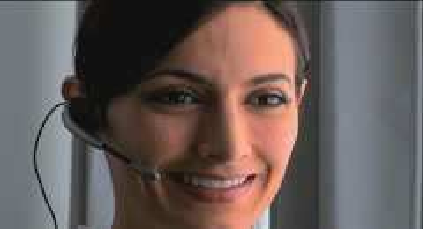
\includegraphics[width=120pt]{images/tm-orig}} \hspace{6mm}
  \subfigure[Cheng 的方法选的点]{
\includegraphics[width=120pt]{images/tm-sel-lc}}
  \hspace{6mm}
  \subfigure[Cheng 的方法着色的结果]{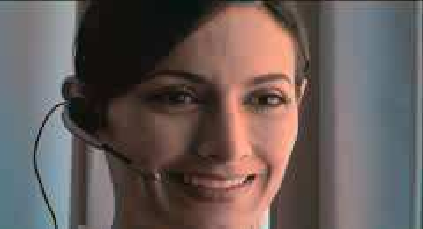
\includegraphics[width=120pt]{images/tm-pred-lc}}\\
  \subfigure[灰度图像]{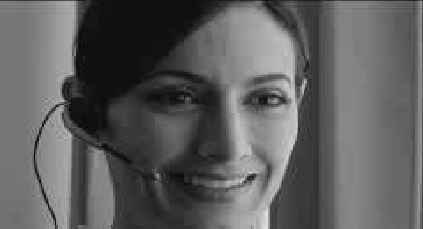
\includegraphics[width=120pt]{images/tm-gray}} \hspace{6mm}
  \subfigure[我们的方法选的点]{
\includegraphics[width=120pt]{images/tm-sel-lap}}
  \hspace{6mm} \subfigure[我们的方法着色的结果]{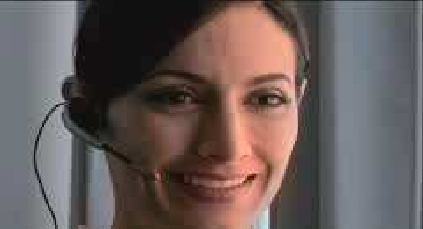
\includegraphics[width=120pt]{images/tm-pred-lap}}
  \caption{\label{fig:tm-compare}第一帧的选点和着色图}
\end{figure*}


  \chapter{结合主动学习和半监督学习的视频压缩}

在本章中我们将介绍如何结合主动学习核半监督学习来进行视频压缩。我们使
用PSNR来衡量图像压缩的质量。

同之前的视频着色和压
缩\cite{learning-to-compress-images,colorization-using-optimization}一
样,我们将使用$YUV$空间。其中$Y$是灰度通道,而$U$和$V$则是存储颜色的色
度通道。我们将独立地预测$U$和$V$两个通道的值。
在\cite{learning-to-compress-images} 中,用于表示一个像素点的特征包括空
间信息和局部的纹理信息。我们经过实验发现局部纹理信息对于预测颜色值来说
并没有什么帮助,因此,我们仅使用空间信息和灰度值来表达每个像素点的特
征。

对于一个一共有$\ell$帧,每一帧有$n$个像素点的视频。首先,我们在第一帧上
应用第 \ref{chap:semi-supervised-learning} 章中所描述的半监督学习算法来
学习一个模型,然后用这个模型来预测该帧以及后续一些帧的颜色值。当PSNR值
低于一定阈值时,我们会重新训练一个模型。半监督学习的过程需要对一一个$m
\times m$的稠密矩阵求逆,这是非常大的计算量。为了减轻计算负担,Chen et
al. \cite{learning-to-compress-images} 建议使用 NCut
\cite{learning-a-classification-model-for-segmentation} 将图像分割成一
些小区域,然后使用 {\em super-pixel} 来表示每个小区域,并在这些小区域
中随机地选择像素点来参与计算。不过 NCut 本身就是一个很耗时的算法。在我
们的工作中,我们采用直接将图像划分为小方格个形式,从而避免了复杂的分割
算法。在我们实验的实验中,我们将小方格的个数定位 2000 个。然后我们会随
机地从每个小方格选取一个像素点,这样总共会有 2000 个像素点,然后我们会
在这些像素点上构造 4-邻接图。

一旦构造好了邻接图,我们就可以应用主动学习的算法来选取最具有代表性的像
素点。视频压缩的质量会随着所选的像素点的数量变化而变化,选的点越多,质
量就会越高。另一方面,选择更多的点会降低压缩比。由于图是在 2000 个点上
构造的,因此最多可以选择 2000 个点。解码的过程就是应用半监督学习算法来
学习一个模型,并用它来预测灰度像素点的颜色值。

\begin{figure*}[t]
  \center \subfigure[Original
  Frames]{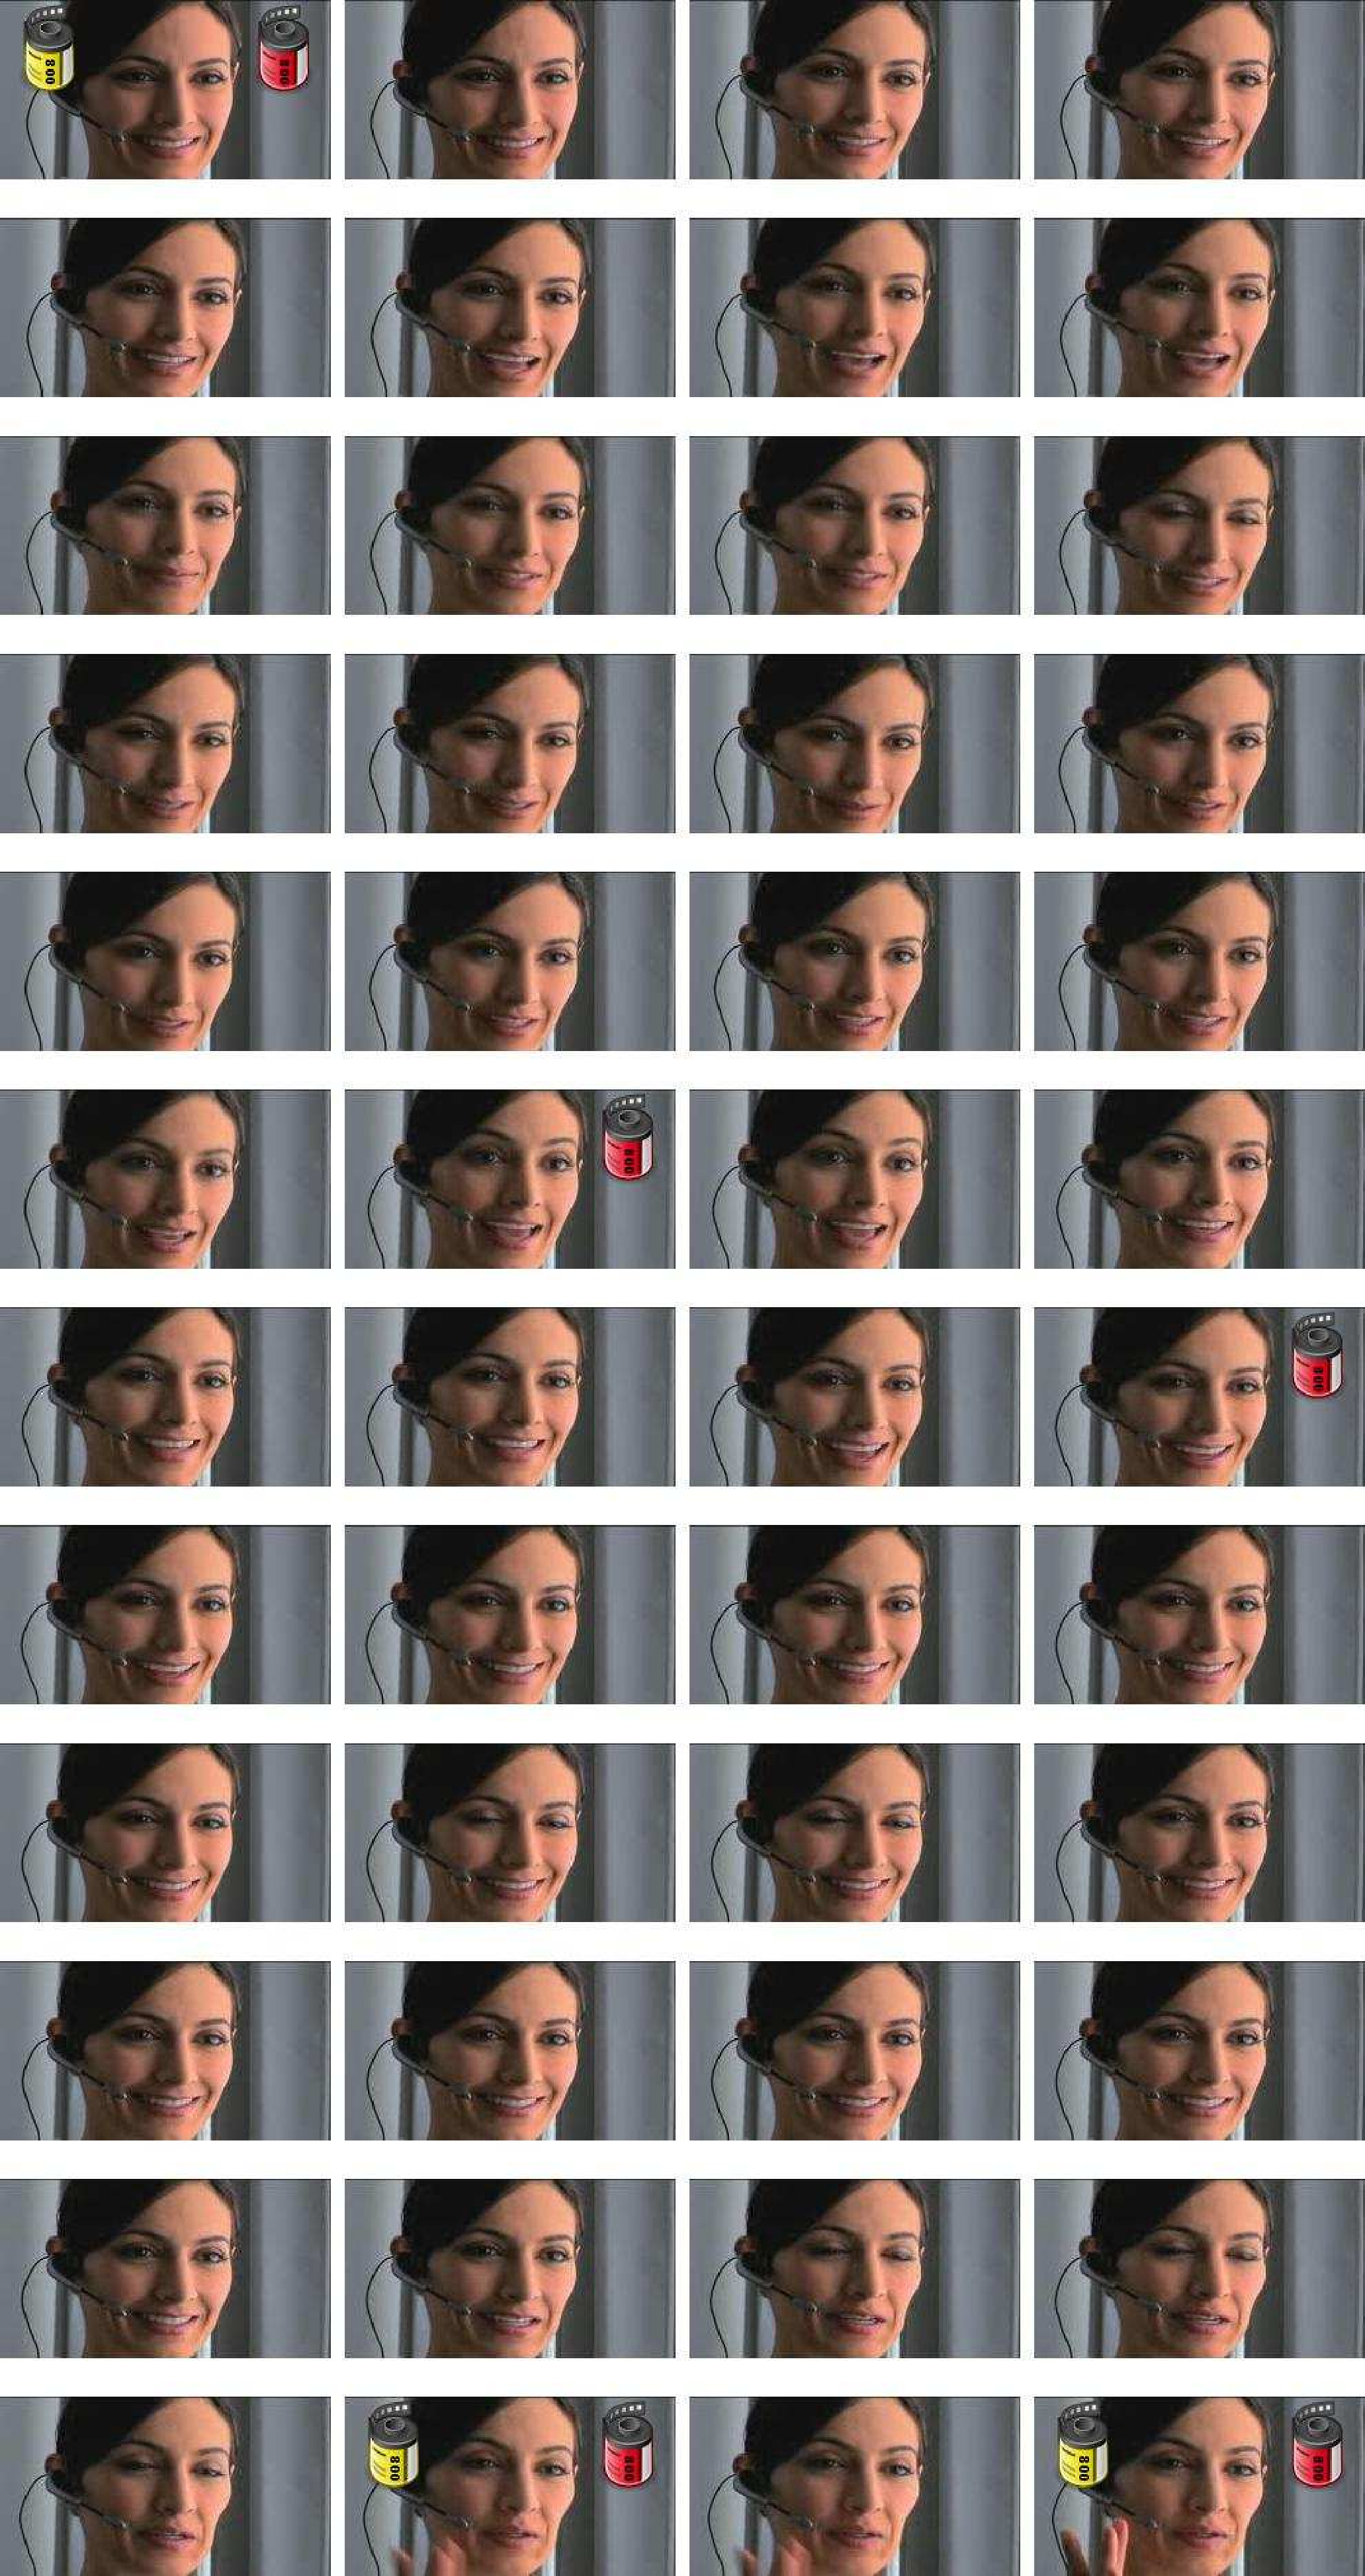
\includegraphics[width=.4\linewidth]{images/telemarket-frames}}
  \hspace{4mm} \subfigure[Colorized
  Frames]{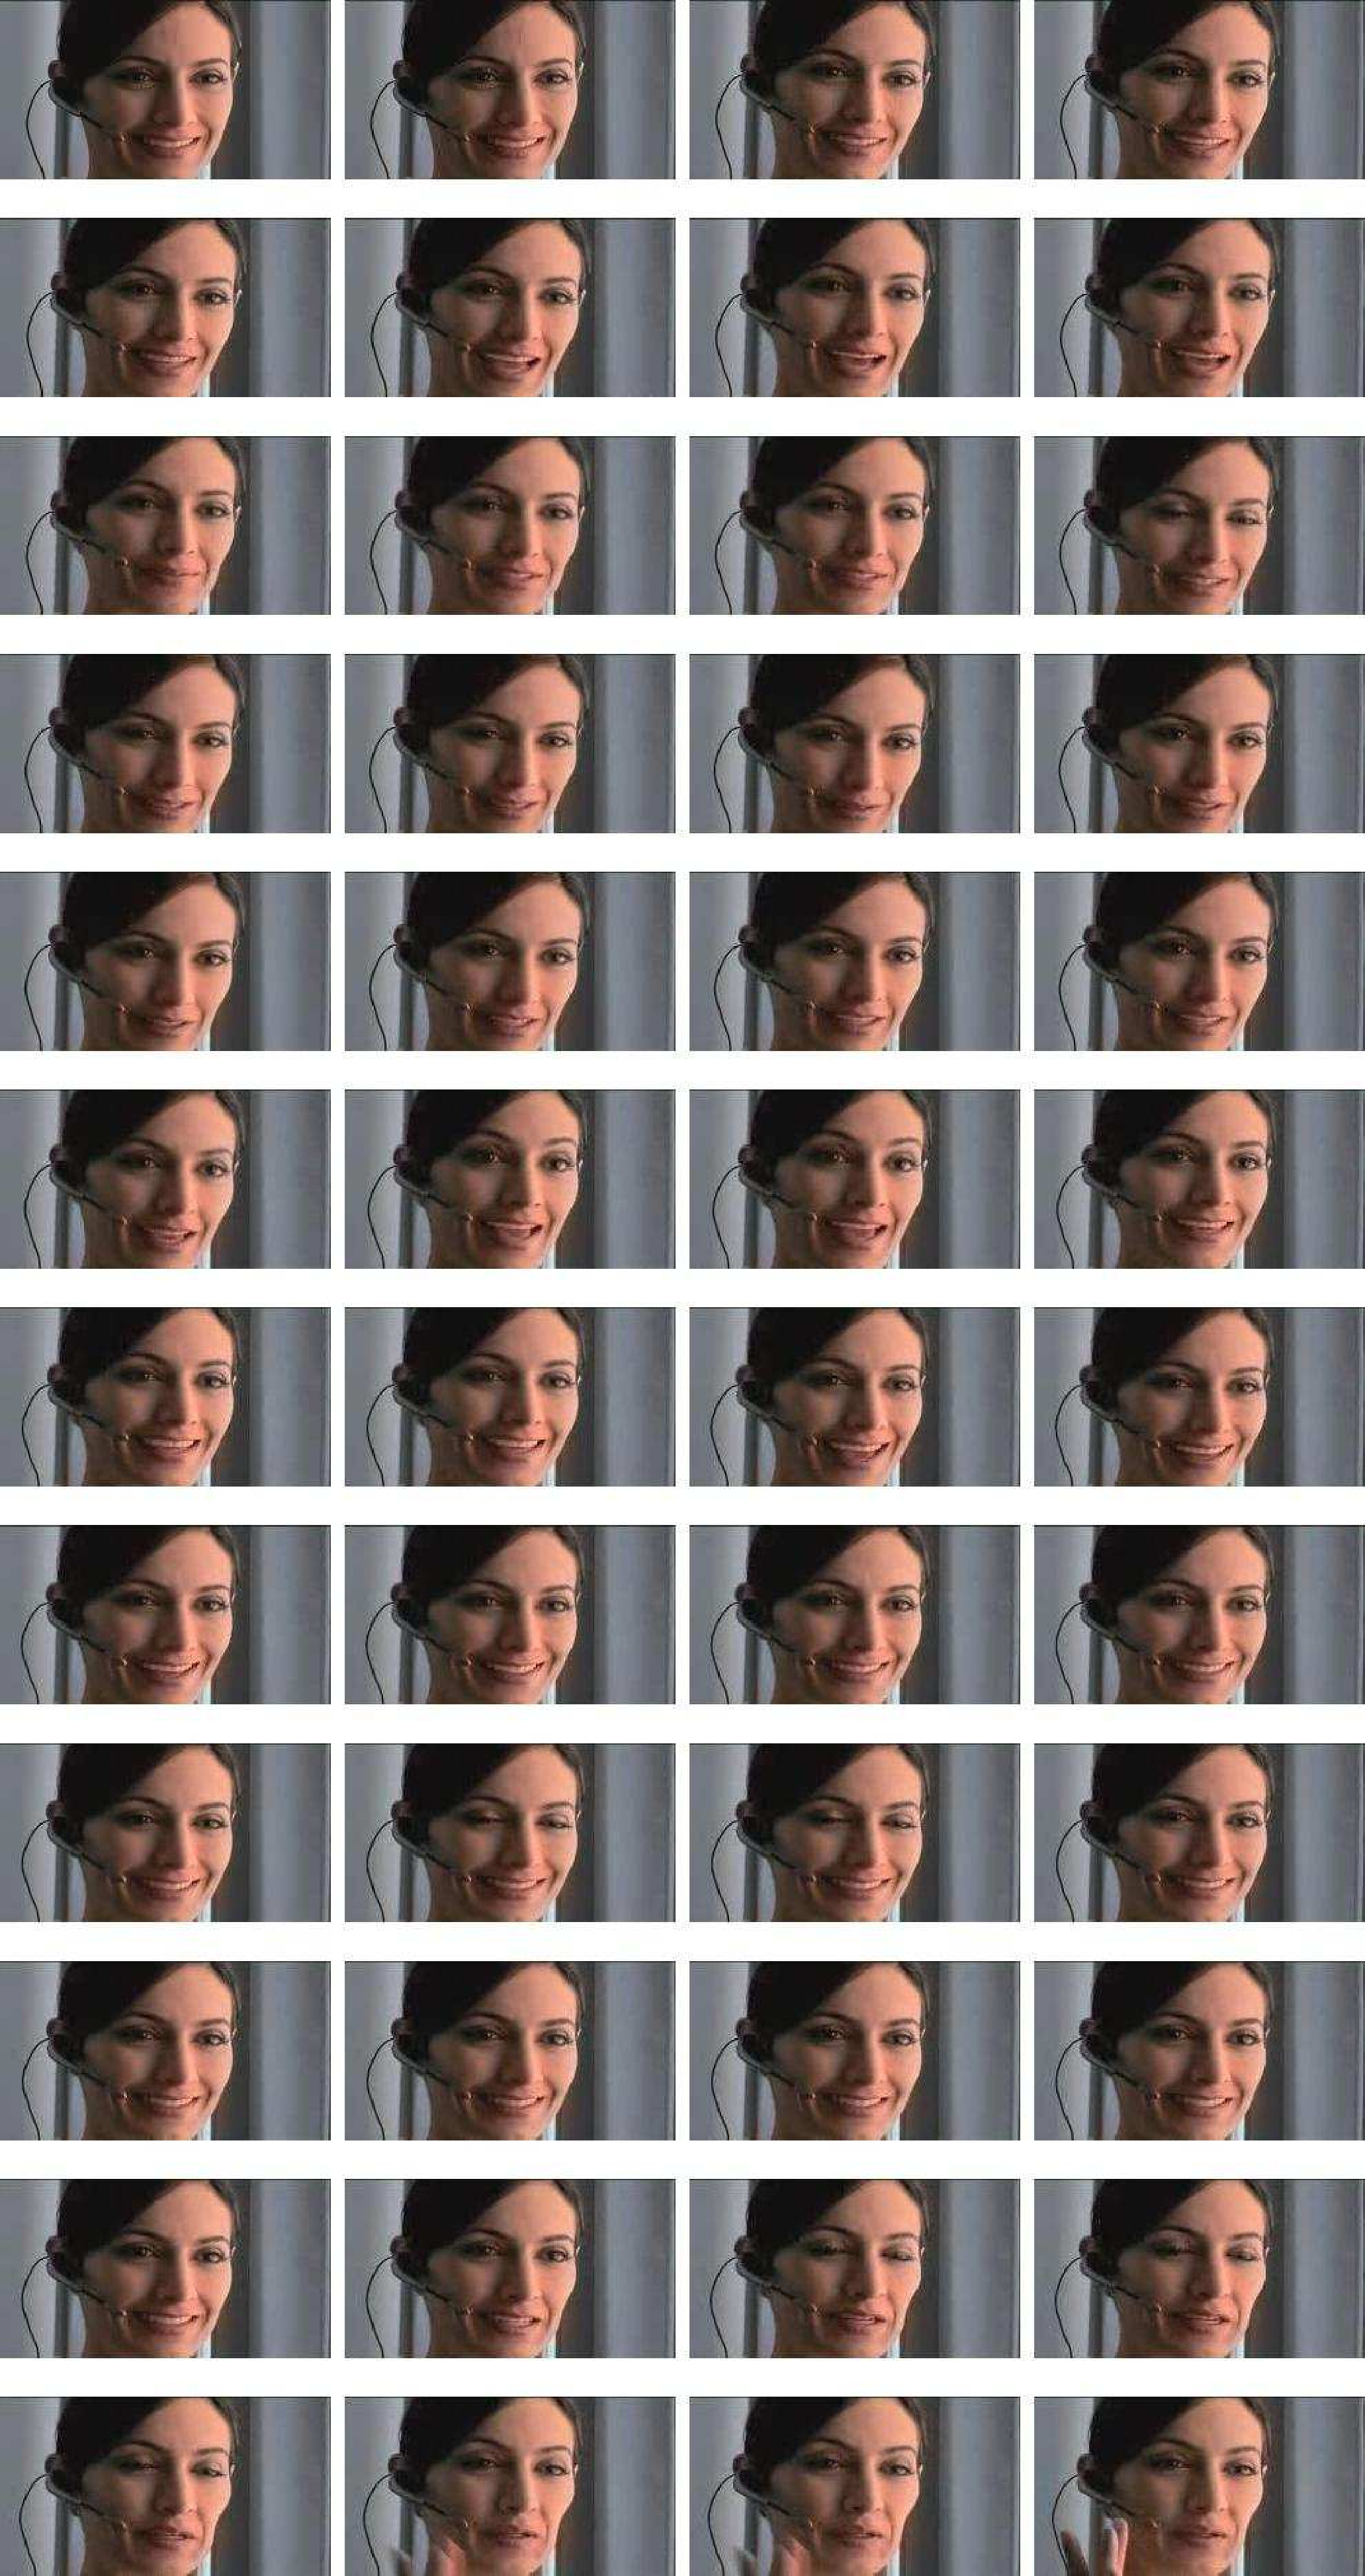
\includegraphics[width=.4\linewidth]{images/telemarket-rcv}}
\caption{The first 48 frames of video
  telemarket. We put a yellow film icon where our method trained a new
  model and a red film icon for Cheng's Approach.}
\label{fig:telemarket}
\end{figure*}


\begin{table*}[t]
  \centering \scriptsize
  \caption{Video compression comparison. cr denotes compression ratio.}
  \label{tab:more-example}
  \begin{tabular}{|l|c|c|c|c|c|c|c|c|c|c|}
    \hline
    video & orig. size & gray. size & \multicolumn{2}{|c|}{Cheng's approach} & \multicolumn{2}{|c|}{SFM} & \multicolumn{2}{|c|}{MFM} & \multicolumn{2}{|c|}{MPEG-4} \\
    \cline{4-11}
    & & & cr & PSNR & cr & PSNR & cr & PSNR & cr & PSNR \\
    \hline
    claire & 463452 & 44556 & 10.48\% & 29.7 & 10.48\% & 35.2 & 10.65\% & \textbf{35.6} & 10.48\% & 35.0 \\
    \hline
    miss-america & 229148 & 17082 & 11.82\% & 35.7 & 11.82\% & 36.4 & 10.60\% & \textbf{37.0} & 11.09\% & 36.0 \\
    \hline
    akiyo & 226780 & 26588 & 12.61\% & 28.3 & 12.61\% & 33.0 & 13.31\% & 33.6 & 12.77\% & \textbf{33.9} \\
    \hline
    suzie & 466278 & 98926 & 34.08\% & 38.5 & 33.23\% & 40.3 & 30.61\% & \textbf{41.1} & 39.29\% & 40.7 \\
    \hline
    mother-daughter & 466836 & 117302 & 28.98\% & 38.2 & 28.55\% & 40.4 & 27.70\% & \textbf{41.2} & 27.54\% & 39.9 \\
    \hline
  \end{tabular}
\end{table*}


  \chapter{实验}

在本章中,我们将评估视频压缩算法的性能。我们同时给了直观的例子和具体的
评估数据。我们使用标准的 PSNR 值作为指标来评估视频压缩质量。

由于一个视频的帧之间不会变化太快,从某一帧训练出来的颜色模型可以直接被
应用到接下来的一些帧上而不会造成太多的视觉上的差异。在我们的实验中,我
们设置一个阈值 $\Delta_{PSNR}$。令 $PSNR^{*}$表示用于训练模型的那一帧的
着色质量,我们将一直使用该模型来预测后续的帧,知道得到的 PSNR 值低
于$PSNR^{*}-\Delta_{PSNR}$为止,此时我们将会重新训练一个模型。因为着色
模型是在单个帧上训练出来的,因此我们把这种方法叫做``单帧模型''(Single
Frame Model, SFM)。最终我们会得到一些着色模型 $SFM_1, \cdots, SFM_k$,
着色模型说对应的那些帧称作关键帧,用 $KF_1, \cdots, KF_k$ 表示。

为了利用视频在时间上的局部性,我们按照下述步骤进一步扩展我们的方法。为
特征空间添加新的一维表示时间的分量$t$,主动学习和半监督学习都将在这个新
的特种空间中进行。与原来使用单帧来训练模型的方法不同,这次我们将同时使
用多个帧来学习,具体地说,我们将关键帧分割为一个一个的时间区间,保证单
个区间内的帧之间的差别不是太大,然后一个区间内的数个关键帧将被用来训练
一个着色模型。我们将这种方法称作多帧模型 (Multiple Frame Model, MFM)。
类似地,我们会得到一系列的着色模型 $MFM_1, \cdots, MFM_l$。需要注意的
是,$MFM_i$仅仅用于预测它所在的那个时间区间内的帧。

\section{选点的评估}

首先我们将在选择最有代表性的点上对比我们的算法和 Cheng 的方法。我们使
用 \cite{learning-to-compress-images} 中使用的那个接线员的视频来进行实
验。该视频一共有 301 帧,每一帧的大小是 $240 \times 130$。

图 \ref{fig:tm-compare}a 和 \ref{fig:tm-compare}d 给出了第一帧和对应的
灰度图像。图 \ref{fig:tm-compare}b 和 \ref{fig:tm-compare}e 分别给出
了Cheng 的主动学习算法和我们的主动学习算法说选出来的像素点。两种算法各
选了 500 个点,可以看到,相比于 Cheng 的算法,我们的方法在颜色改变的边
界处选择了更多的点,从我们的算法选出来的点的分布可以大致看出一个人脸的
轮廓。图 \ref{fig:tm-compare}c 和 \ref{fig:tm-compare}f 给出了 Cheng
和我们的方法着色(和解压缩)的结果。可以看到,我们的方法给出了视觉上更
好的结果。对于第一帧,Cheng 的方法得出的 PSNR 是 $35.38$,我们的方法是
$38.99$,比 Cheng 的方法明显要高。

\section{视频压缩质量的评估}

这个实验的目的是从视频压缩的质量上来比较我们的方法和 Cheng 的方法。通过
固定总的选点数目的办法,我们将压缩比设定为一个固定值,有此通过比较
PSNR 值的办法来衡量视频压缩的质量。

在视频压缩的过程中训练的模型的个数依赖于 $\Delta_{PSNR}$ 和着色的质量。
在这个实验中,Cheng 的方法一共训练了 9 个模型,而我们的 SFM 和 MFM 方
法分布训练了 9 个和 3 个模型。要让各个方法选点的总数完全一样几乎是不可
能的事,对于 Cheng 的方法,每次重新训练模型的时候都会选择 500 个点,因
此一共选择了 4500 个点,我们的 SFM 也是一样,因此一共也是选择了 4500
个点,而对于 MFM 来说,我们并没有将每次选点的个数设定为一个固定值,而
是选择足够多的点,使得其 PSNR 值不会低于 SFM ,在这个实验中,MFM 所选
点的总数是 3900 。

我们使用 {\em MPlayer's Movie Encoder} 来将原始视频编码为 MPEG-4 的格
式,占用的大小为 756,586 字节。然后我们用同样的编码方式将该视频编码为灰
度格式,得到的结果占用 250,288 字节。该灰度视频会在解码的时候用到。为
了恢复灰度视频,除了灰度视频之外,我们还需要存储选出来的点的空间信息和
颜色值。因此,我们需要额外的 4 个字节来存储每一个选定的点的信息(2 个
字节来存储颜色信息,2 个字节存储位置信息)。因此,Cheng 的方法和 SFM
都需要额外 18,000 字节的存储空间,而 MFM 只需要 15,600 字节。

在图 \ref{fig:telemarket}a 中,我们给出了原始视频的 48 帧,黄颜色的标记
标识了我们的算法训练模型的帧,而红色的标记则标识了 Cheng 的算法训练模型
的帧。可以看到,在第二个红色的标记的地方(第 6 行,第 2 列),该帧和前
面的帧的差别并不是特别大,然而 Cheng 的方法却在这里选择重新训练一个模
型,这是不必要的。相比起来,对于每个黄颜色的标记,我们都可以看到对应的
帧和其之前的帧是有比较大的差别的,我们的算法只在这些帧上训练新的模型。
图 \ref{fig:telemarket}b 给出了我们的方法所恢复出来的视频的对应帧。

为了比较不同算法的视频压缩的质量,我们在图 \ref{fig:psnr-more}a 中画出
了每一帧的 PSNR 值,其中横坐标是视频的帧,而纵坐标是对应的帧所恢复出来
的结果的 PSNR 值。我们还在训练模型的帧所在的地方绘制了实心圆,并且圆的
大小正比于该模型选点的数目。可以看到,在总的选点数差不多相等(亦即压缩
比相等)的情况下,我们的 SFM 和 MFM 给出的 PSNR 值比 Cheng 的方法要高许
多。具体来说,Cheng 的方法、我们的 SFM 还有 MFM 所得到的 {\em overall}
PSNR \cite{wavelet-based-rate-scalable-video-compression}值分别
是 $34.8$,$38.0$和$38.4$。

表格 \ref{tab:more-example} 给出了一些其他的视频压缩的结果\footnote{所
  有的视频都可以在 \url{http://trace.eas.asu.edu/yuv/index.html} 下载
  到。},对应的 PSNR 图也可以在图 \ref{fig:psnr-more} 中找到。在这里我
们同时还比较了标准的 MPEG-4 视频压缩的结果,我们将原始视频用标准的
MPEG-4 编码器压缩到一个差不多的压缩率,然后计算结果的 PSNR 。从表中可
以看到,在压缩比差不多的情况下,我们的方法可以得到的 PSNR 比 Cheng 的
方法要高许多,并且有时候比标准的 MPEG-4 还要好。

\begin{figure*}[t]
  \centering
  \subfigure[telemarket]{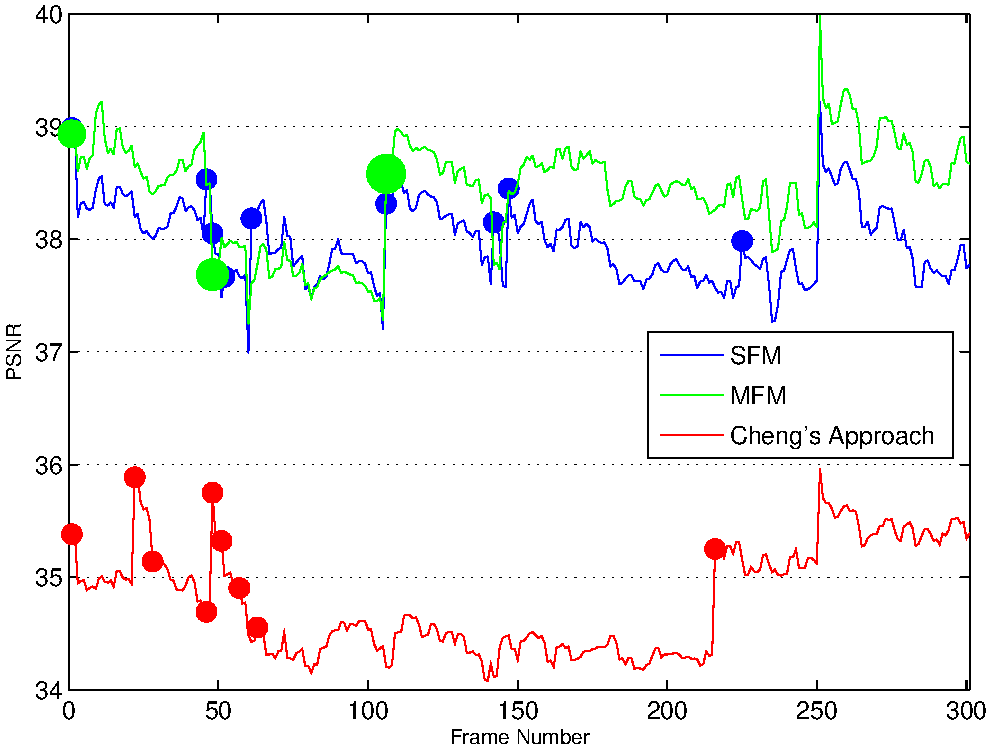
\includegraphics[width=.4\linewidth]{images/telemarket}}
  \subfigure[claire]{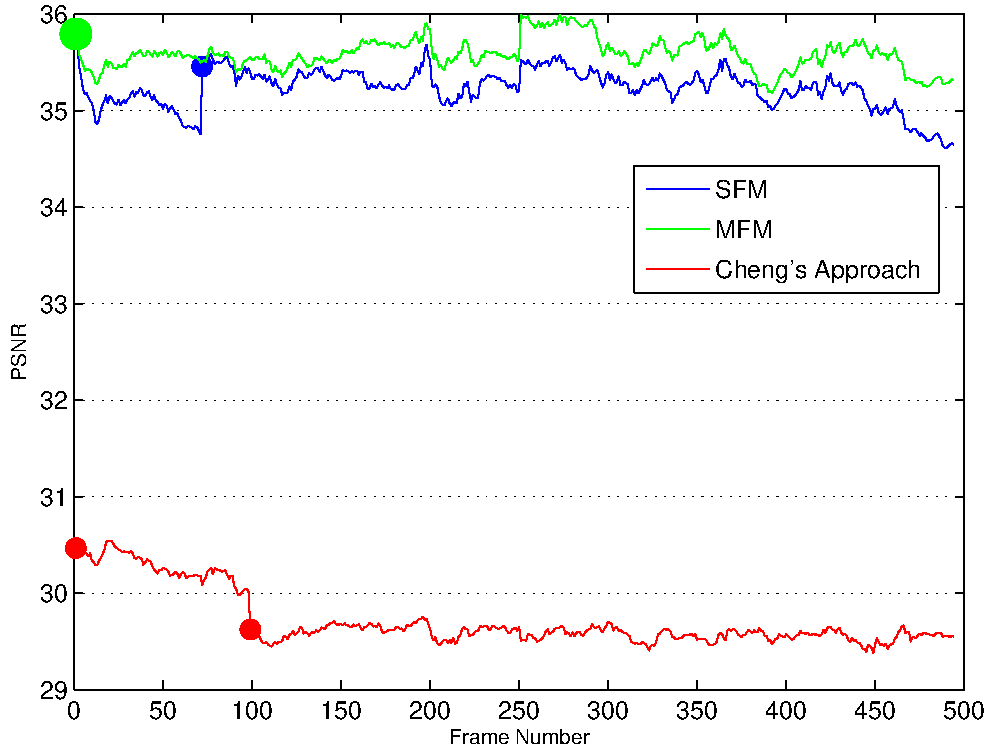
\includegraphics[width=.4\linewidth]{images/claire}}
  \subfigure[miss-america]{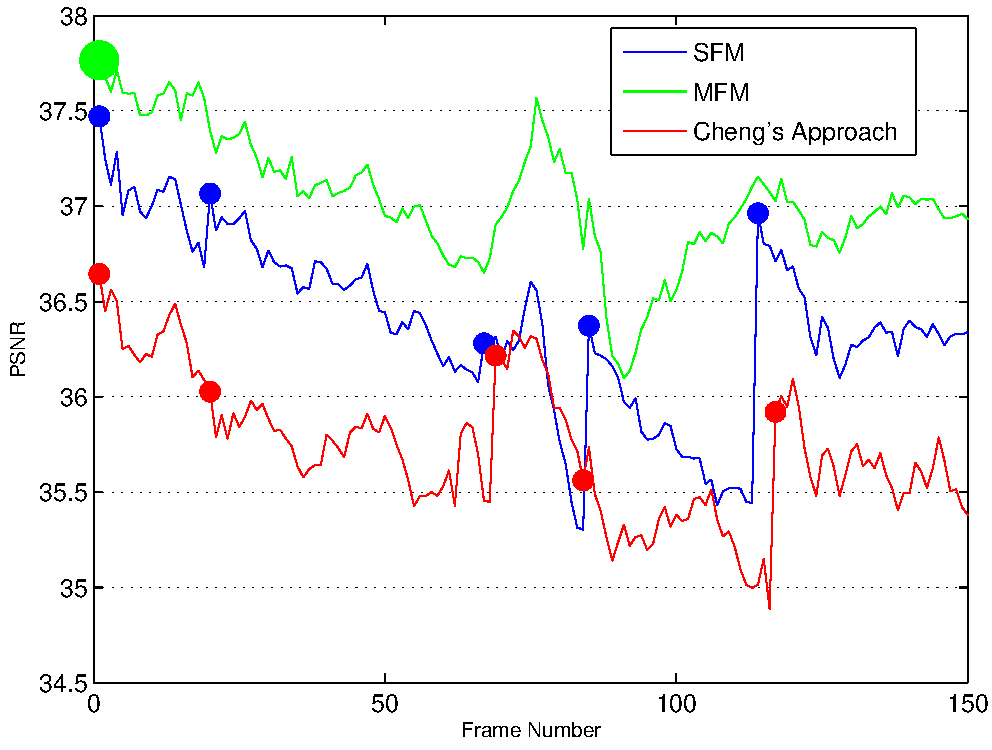
\includegraphics[width=.4\linewidth]{images/miss-america}}
  \subfigure[akiyo]{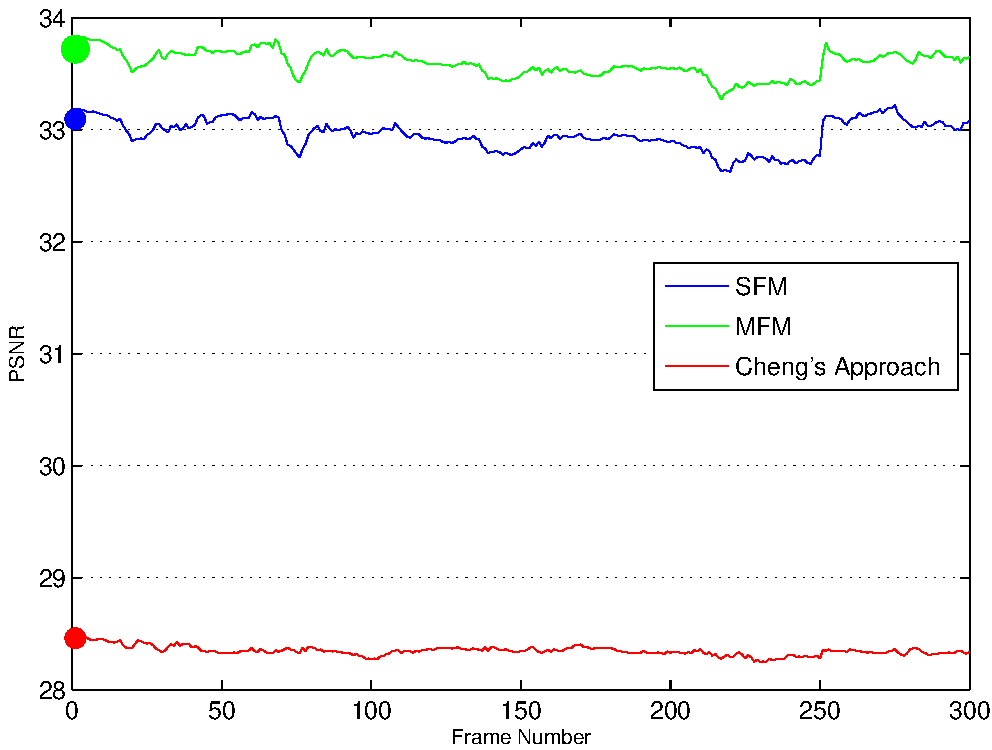
\includegraphics[width=.4\linewidth]{images/akiyo}}
  \subfigure[suzie]{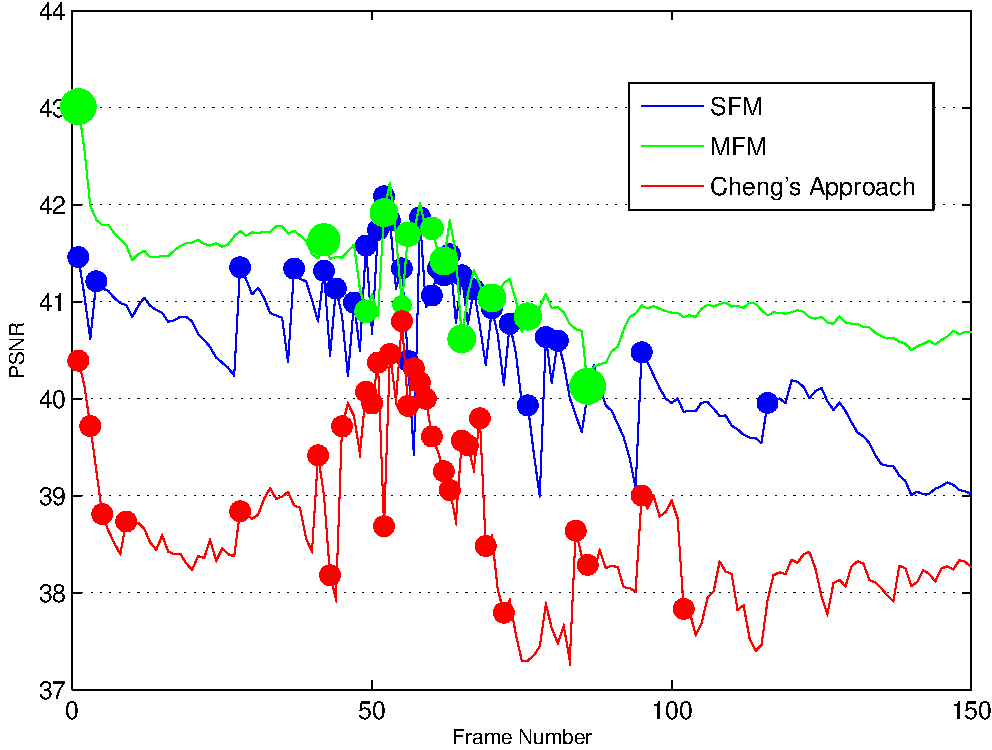
\includegraphics[width=.4\linewidth]{images/suzie}}
  \subfigure[mother-daughter]{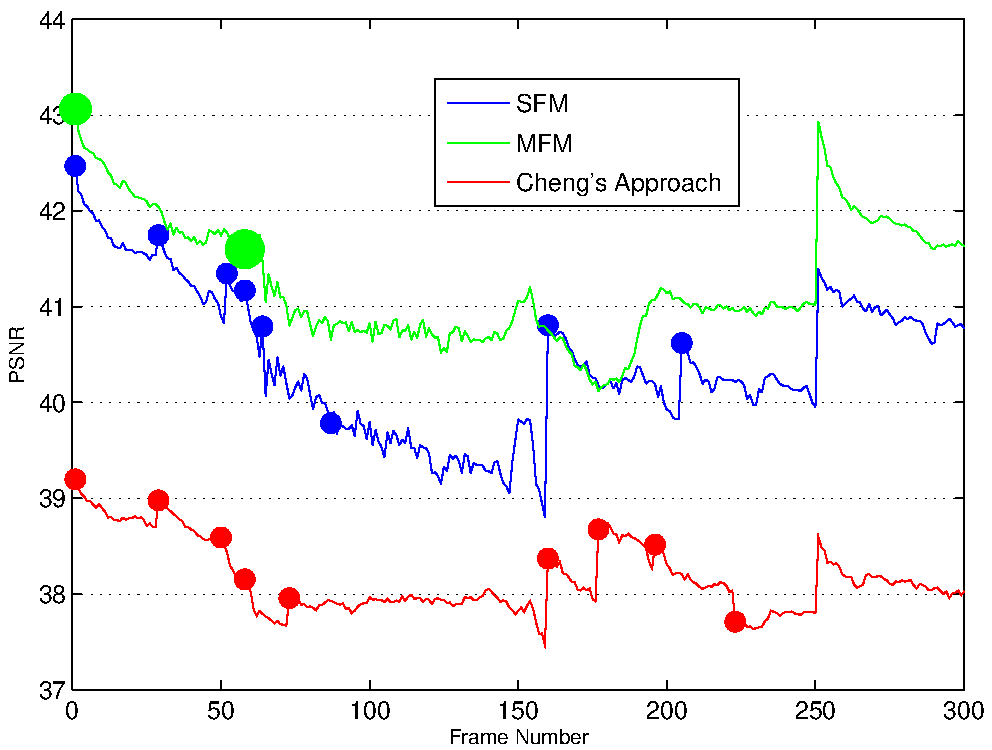
\includegraphics[width=.4\linewidth]{images/mother-daughter}}
  \caption{The PSNR plots. For all these examples, our approach obtains significantly higher PSNR than Cheng's approach.}
\label{fig:psnr-more}
\end{figure*}


  \chapter{结论和展望}

我们给出了一个用于视频压缩的统一的主动学习和半监督学习的框架。给定的算
法的灵感来源于基于图的半监督学习的最新进
展 \cite{Manifold-Regularization-Journal}。使用最优化实验设计的技术,我
们通过最小化系数的协方差矩阵的方式来进行选点。对于视频压缩来说,主动学
习的方法将会用于选取最有代表性的像素点,而半监督学习则会用于着色的过
程。实验结果显示我们的方法的性能地超过了目前的其他方法。

我们希望这里提出的算法和框架可以提供一个图像和视频分析的新的视角。这篇
论文主要集中在视频压缩上,但是,相同的思想可以被应用到其他类似的问题
上,例如重要区域检测。



%==============================================================
%这也是个不需要自己修改的部分。

  \backmatter %结束章节自动编号

  %参考文献
  \addcontentsline{toc}{chapter}{参考文献} % 解决目录中没有相应的参考文献的条目问题
  \chaptermark{参考文献}

%==============================================================

  \bibliography{data/zjubib}

  %致谢
  %致谢
\chapter*{\centerline{致\quad 谢}}
\chaptermark{致谢}
\addcontentsline{toc}{chapter}{致谢}

\vspace{2em}


  %附录
  \chapter*{附\quad 录}
\chaptermark{附录}
\addcontentsline{toc}{chapter}{附录} 


  %任务书
  %任务书
\chapter*{\centerline{\stxingkai\erhao 本科生毕业论文(设计)任务书}}
\thispagestyle{empty}

\vspace{2em}

{\stfangsong\xiaosi\bf
一、\;题目:\;\underline{\songti\zjutitlec}

二、\;指导教师对毕业论文(设计)的进度安排及任务要求:
\vspace{4cm}

\begin{flushright}
起讫日期 200 \quad 年 \quad 月 \quad 日 至 200 \quad 年 \quad 月 \quad 日\\
指导教师(签名)\;\underline{\hspace{4em}} \quad 职称\;\underline{\hspace{4em}}
\end{flushright}

三、\;系或研究所审核意见:
\vspace{4cm}
\begin{flushright}
负责人(签名)\underline{\hspace{4em}}\\
\quad 年 \quad 月 \quad 日
\end{flushright}
}

  %考核
  %考核
\chapter*{\centerline{\stfangsong\xiaoer 毕~业~论~文~(设计)~考~核}}
\thispagestyle{empty}

\vspace{2em}

{\stfangsong\sihao\bf
一、\;指导教师对毕业论文(设计)的评语:
\vspace{4cm}

\begin{flushright}
    指导教师(签名)\;\underline{\hspace{4em}}\\
    年\quad 月\quad 日
\end{flushright}

二、\;答辩小组对毕业论文(设计)的答辩评语及总评成绩:
\vspace{4cm}

{\songti\xiaosi
\begin{tabular}{|c|c|c|c|c|c|}
    \hline
    成绩比例 & \parbox[t]{4em}{文献综述\\[-3.5em]占(10\%)} & 
               \parbox[t]{4em}{开题报告\\[-3.5em]占(20\%)} & 
               \parbox[t]{4em}{外文翻译\\[-3.5em]占(10\%)} &
               \parbox[t]{7em}{毕业论文(设计)\\[-3.5em]质量及答辩\\[-3.5em]占(60\%)} & 
               总评成绩 \\
    \hline
    分值 & & & & & \\
    \hline
\end{tabular}
}

\begin{flushright}
    答辩小组负责人(签名)\;\underline{\hspace{4em}}\\
    年 \quad 月 \quad 日
\end{flushright}
}


%==============================================================
%==============================================================
\end{document}
